As Schol\'e AI is still in its early development phase, we currently do not have access to real-world user data. To lay the foundation for experimentation and model training, we first established a formal typology of the types of data that will characterize student profiles. We categorized the data into two primary types: explicit data and implicit data.

\paragraph{Explicit Data.}  
This category encompasses all directly stated learner preferences and declared learning goals. It includes information such as preferred learning modalities, self-reported motivation, goal orientation, or feedback explicitly given by the learner regarding content relevance or difficulty. These data points are directly interpretable. The detailed categories can be found in Appendix~\ref{appendix:explicit_data}.

\paragraph{Implicit Data.}  
Also referred to as \textit{behavioral data}, this category includes information derived from the learner's interaction patterns with the learning system. Behavioral data captures observable signals such as time spent on tasks, content navigation paths, click-through rates, quiz completion rates, and error frequencies. The detailed categories can be found in Appendix~\ref{appendix:implicit_data}.

\section{Prompt Engineering}

\subsection{System prompt} The system prompt is responsible for guiding the model by specifying the overall structure, formatting, and style of the generated output. Unlike the user prompt, it remains constant across generations.

We implemented a synthetic data generation pipeline built upon prompt engineering techniques, following the methodology presented in \cite{sahoo2025systematicsurveypromptengineering}. We adopted the   \textbf{in-context learning} (ICL) \cite{dong2024surveyincontextlearning} with \textbf{one-shot prompting}, enabling the model to produce with simplicity structured and context-aware outputs. 

\textit{In-context learning} is a paradigm that allows language models to learn tasks given only a few examples in the form of demonstration. This allows the model to adapt its behavior based on the structure and semantics of the provided context. Specifically, we use one-shot prompting, where the model is provided with a single example before generating its output. Since prompts can become lengthy quickly, this approach offered a good compromise between clarity and conciseness.

Each system prompt is structured as follows:
\begin{itemize}
	\item A definition of the task (three possibilities: synthetic data generation, data augmentation, or curriculum pairs generation).
    \item A subgraph extracted from Scholé AI's main \textit{knowledge graph} (KG), describing learning modules. This ensures that the model grounds its generation in the actual curriculum.
    \item A strict requirement to output data in a structured \texttt{JSON} format, which enables automatic validation and downstream processing.
\end{itemize}

Since the initial KG contained 415 nodes, we applied several techniques to extract the most relevant concepts. We tested methods like Betweenness Centrality, PageRank, and Strongly Connected Components. The one producing the best results to capture the most important concepts was Betweenness Centrality, which measures how often a node appears on the shortest paths between other nodes. We selected the 25 most relevant modules for the prompt, as illustrated in Figure~\ref{fig:graph}.
\begin{figure*}[h!]
	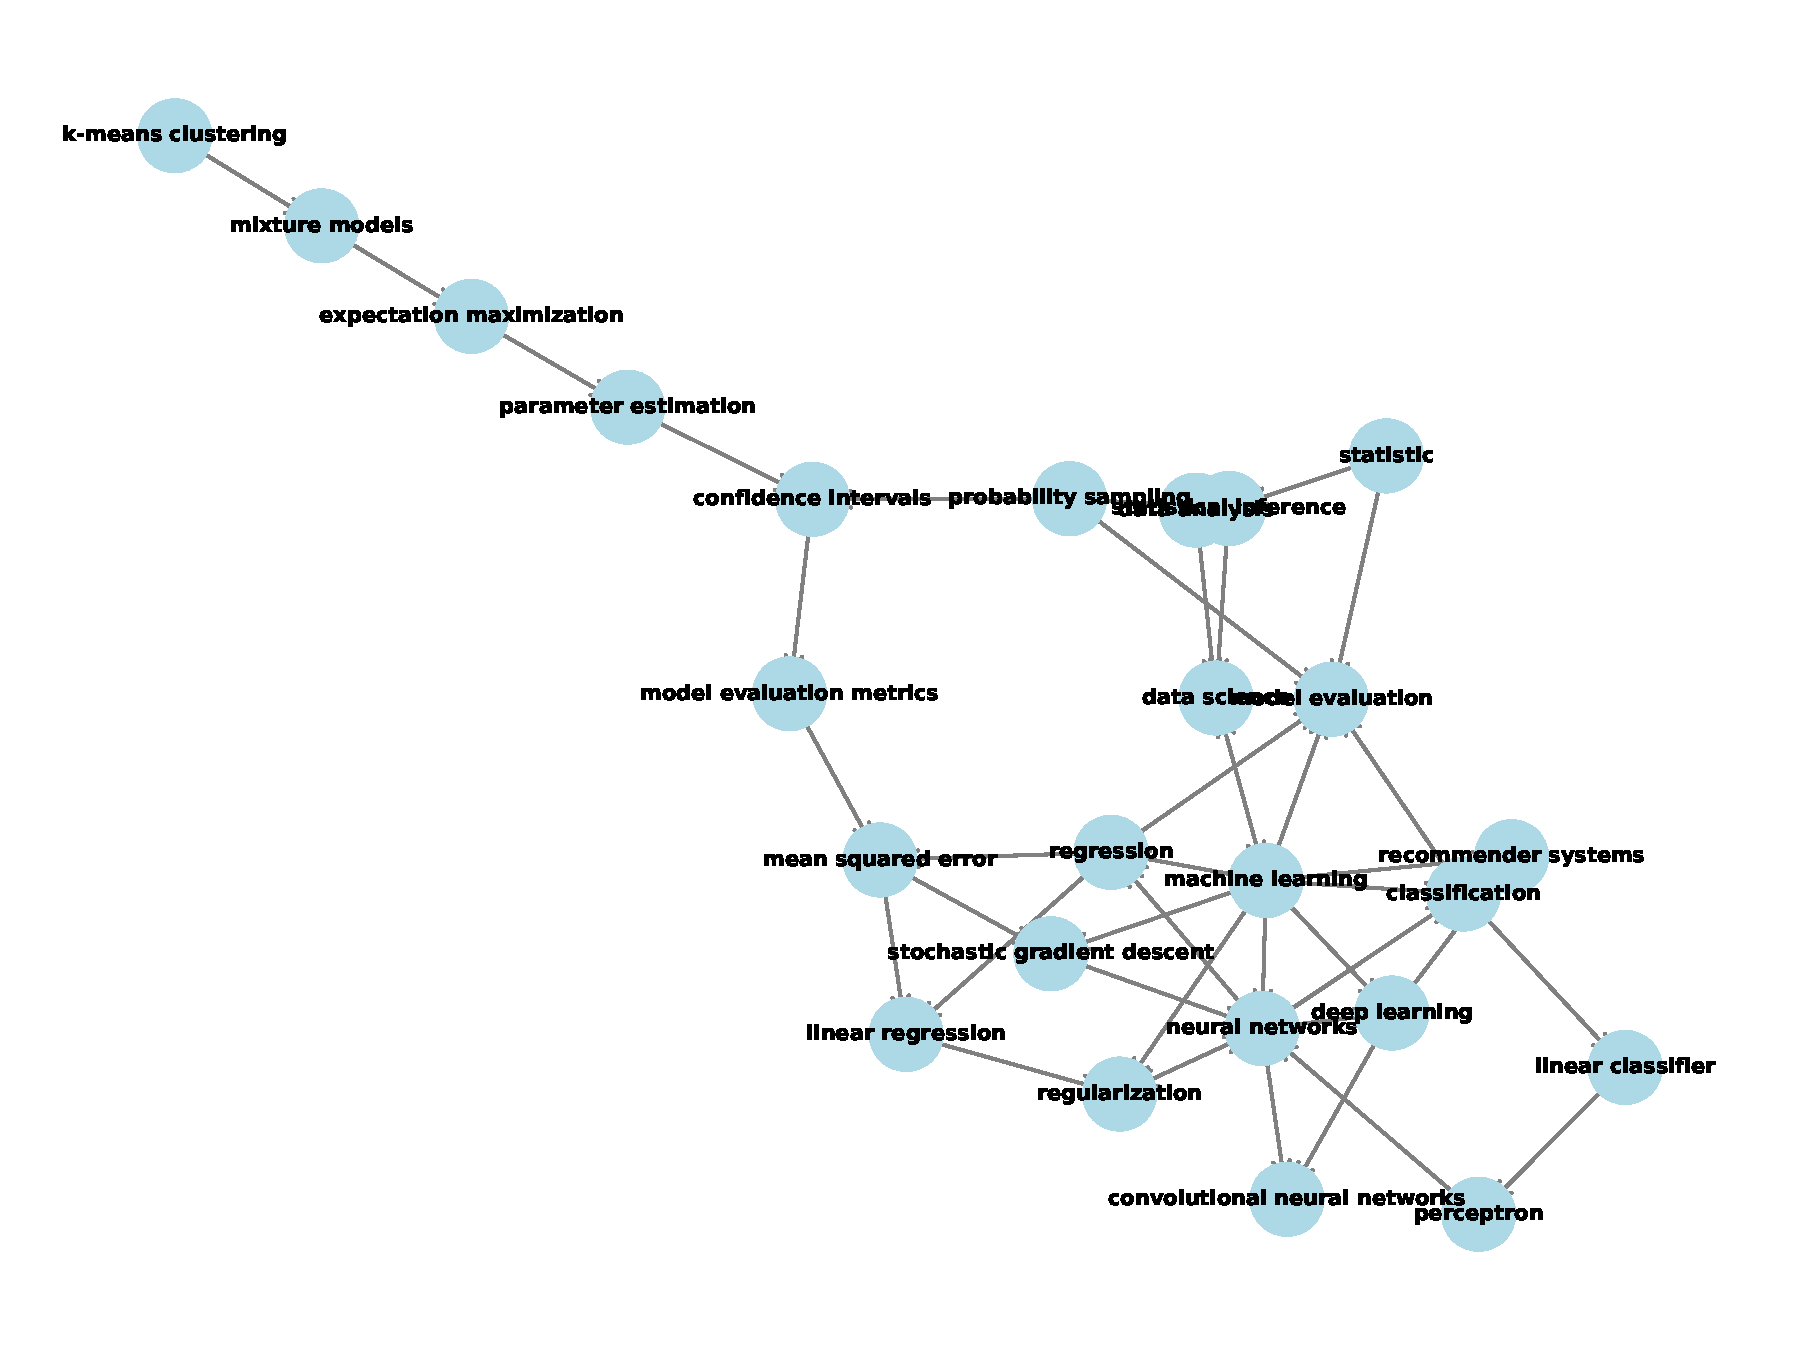
\includegraphics[width=\textwidth]{scholeai_betweenness_summary.pdf}
  \caption{ScholéAI Knowledge Graph (Top-25 nodes by Betweenness Centrality).}
  \label{fig:graph}
\end{figure*}

For more details, the prompts used for the three tasks — Synthetic Data Generation, Data Augmentation, and Curriculum Pairs Generation — can be found in Appendix~\ref{appendix:prompt1}, Appendix~\ref{appendix:prompt2} and Appendix~\ref{appendix:prompt3} respectively.

\subsection{User prompt} In the Synthetic Data Generation task, to introduce diversity we incorporate personalization into the user prompt with the learning modality and student profile. This prompt also specifies the number of generations to produce.

\paragraph{Learning Modalities.}  
We defined the following learning modalities to reflect common cognitive styles according to the VARK model:

{\small
\begin{itemize}
    \item \textit{Visual}: prefers diagrams, illustrations, and video content.
    \item \textit{Auditory}: favors spoken explanations, podcasts, and discussions.
    \item \textit{Reading/Writing}: learns through text-based material such as articles and notes.
    \item \textit{Kinesthetic}: benefits from interactive, hands-on experiences.
\end{itemize}
}

It's worth noting that these modalities can be somewhat controversial, which is why they should be used with caution \cite{vark-casestudy}. Nonetheless, we adopt them in the early stages due to their simplicity.

\paragraph{Student Profiles.}  
We define several learner types to reflect diverse engagement styles:

{\small
\begin{itemize}
\item \textit{Goal-Oriented}: driven by milestones and performance tracking.
\item \textit{Curious}: explores optional content and asks open-ended questions.
\item \textit{Passive}: minimal engagement, avoids extra effort.
\item \textit{Fast-Paced}: skims content, prioritizes speed over depth.
\item \textit{Confused}: struggles with core concepts, needs clear guidance.
\item \textit{Struggling}: performs poorly, benefits from scaffolding and feedback.
\item \textit{Social}: learns through discussion and peer interaction.
\end{itemize}
}

For the Data Augmentation and Curriculum Pairs Generation tasks, the user prompt serves a different purpose: it provides the input \texttt{JSON} data, which the model either augments or uses to generate personalized learning plans.

In the Figures \ref{fig:diag1} and \ref{fig:diag2} below, you can find diagrams to summarize the structure of the different prompts.

\newpage
\begin{figure*}[h!]
	\center
	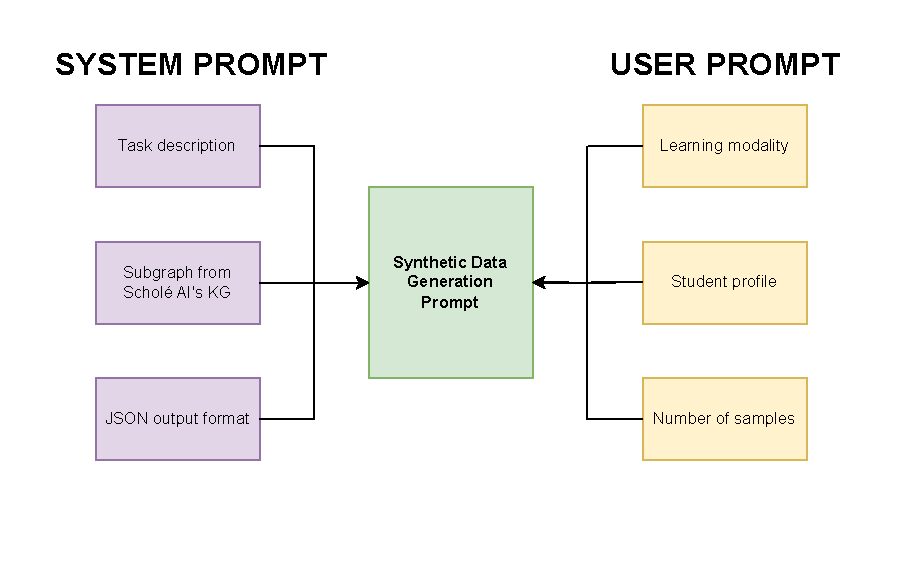
\includegraphics[width=0.9\textwidth]{Diag1.pdf}
  	\caption{Summary diagram for the Synthetic Data Generation prompt.}
  	\label{fig:diag1}
\end{figure*}

\vspace{1cm}

\begin{figure*}[h!]
	\center
	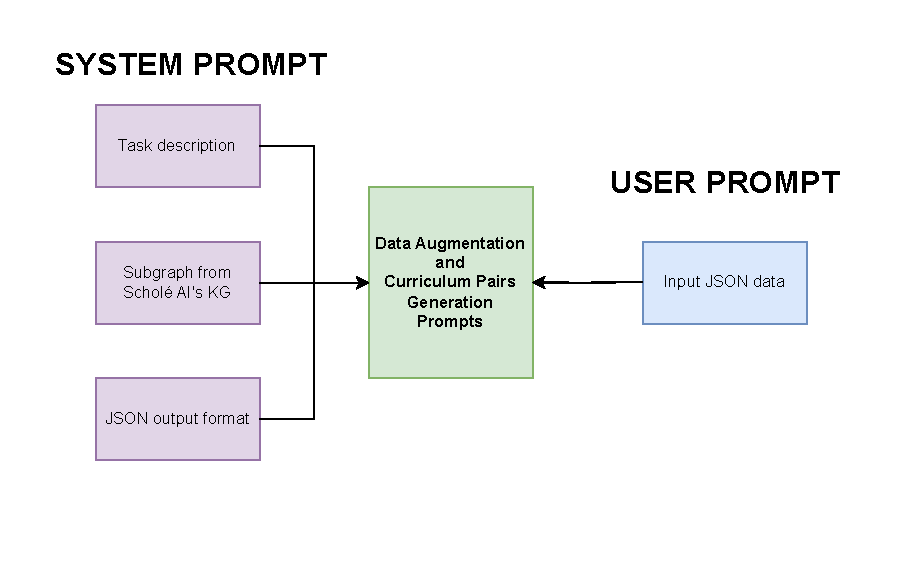
\includegraphics[width=0.9\textwidth]{Diag2.pdf}
  	\caption{Summary diagram for the Data Augmentation and Curriculum Pairs Generation prompts.}
  	\label{fig:diag2}
\end{figure*}

\vspace{1cm}
The latest versions of the prompts are available in \texttt{JSON} format at \href{https://github.com/JCHAVEROT/semester-project/tree/main/experiments/SyntheticData/prompts}{this link}.


\newpage

\section{Streamlit Interface for Prompt Interaction}

To support fast iterations on prompt design and inference control, we developed an interactive interface using \textbf{Streamlit}.

\textit{Streamlit} is an open-source Python framework that enables rapid development of web applications for data science and machine learning tasks. It allows users to manipulate model inputs and visualize outputs without requiring front-end development.

Our Streamlit interface provides the following features:
\begin{itemize}
	\item Choosing the task type.
	\item Editing prompt content in real time.
	\item Selecting learning modalities and student profiles.
	\item Evaluating the generated synthetic data.
% \item Adjusting generation parameters such as temperature, top-$p$, and model choice.
\end{itemize}

The website can be accessed at this link: \href{https://https://data-for-scholeai.streamlit.app/}{https://https://data-for-scholeai.streamlit.app/}

\begin{figure*}[h!]
	\center
	
\includegraphics[width=\textwidth]{screen1.png}
  	\caption{Screenshot of the Streamlit web app home page.}
  	\label{fig:screen1}
\end{figure*}

Screenshots of the user interfaces (UIs) can be found in Appendices \ref{appendix:screen1}, \ref{appendix:screen2}, \ref{appendix:screen3}, \ref{appendix:screen4}, \ref{appendix:screen5} and \ref{appendix:screen6}.

\section{Evaluation Pipeline: Automated and Human-in-the-Loop}

Once the synthetic data pipeline was functional, the next challenge was to assess the quality of the generated outputs. We implemented an evaluation process with two layers combining automated validation and expert evaluation.

\subsection{Automated Evaluation}  
Given the structured nature of the outputs, we first applied a series of automated validation tests to each generated \texttt{JSON} sample. These included the following checks, among others:
\begin{itemize}
    \item All required fields were present and of the correct type.
    \item Categorical values (e.g., learning modality) belonged to the expected set.
    \item Text fields were non-empty where applicable.
    \item Timestamps respected ISO 8601 formatting and logical sequencing.
    \item Numeric ratings fell within predefined bounds (e.g., 1--5).
\end{itemize}

These tests served as an efficient first-pass filter, rejecting malformed samples before any human review. The complete list of tests can be found in Appendix~\ref{appendix:validation_checks} and the UI in Appendix~\ref{appendix:screen5}.

\subsection{Human Evaluation via Yes-No Questions}  
For semantic and pedagogical validity, we developed a human annotation interface embedded on the Streamlit web app. Annotators assessed each sample using a series of \textit{yes-no questions}, such as:
\begin{itemize}
    \item Is the proposed curriculum realistic for the given student profile?
    \item Does the plan match the specified learning modality?
    \item Is the behavioral data coherent and believable?
\end{itemize}

This human-in-the-loop component allowed for rapid, structured assessment without requiring full expert review. The feedback was used to iteratively improve prompt design and increase generation quality. The full list of questions is provided in Appendix~\ref{appendix:questions} and the UI in Appendix~\ref{appendix:screen6}.

\subsection{Visualization of Evaluation Results}
  
To monitor performance and guide refinements, we use the Plotly library to produce interactive dashboards summarizing evaluation statistics for automated checks and human questions.
These summaries offered useful feedback on the effectiveness of the prompts and played a key role in refining them and monitoring progress over time.

For example in Figure~\ref{fig:plot1} are shown some automated results for 10 synthetic samples generated through the web app. In Figure~\ref{fig:plot2} are some results for the expert validation.

The evaluation tool helped identify areas where the prompt needed improvement. For instance at the beginning, timestamp fields often failed to follow the ISO 8601 format. We revised the prompt to clarify this requirement and remove ambiguity.

The tool was also helpful when we noticed that including a full real sample in the prompt led the model to repeat parts of it in the outputs. We updated the prompt to show the full \texttt{JSON} structure as an example, but left the fields empty to avoid content leakage.

\newpage

\begin{figure*}[h!]
	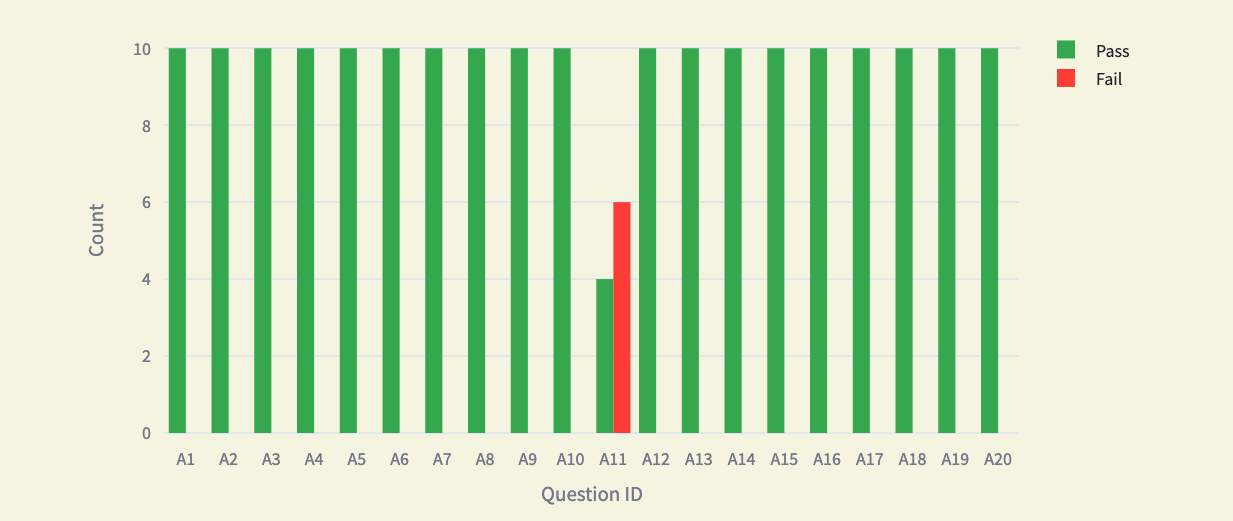
\includegraphics[width=\textwidth]{plot}
  \caption{Summary statistics for the automated tests.}
  \label{fig:plot1}
\end{figure*}

\vspace{3cm}

\begin{figure*}[h!]
	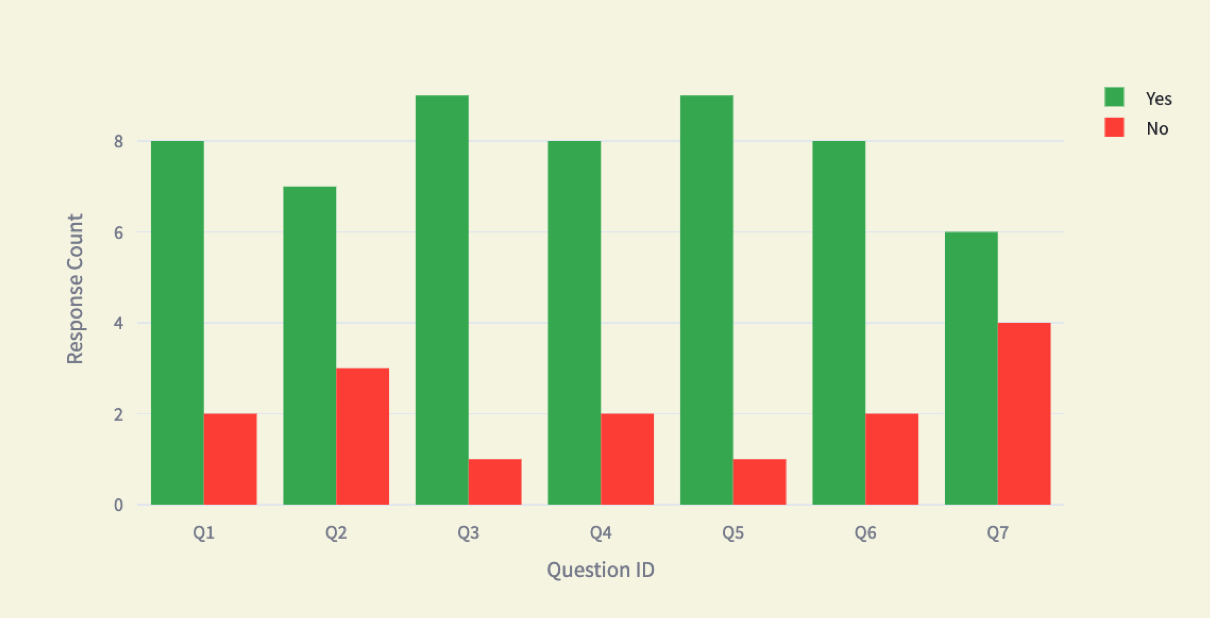
\includegraphics[width=\textwidth]{plot2}
  \caption{Summary statistics for the expert evaluation.}
  \label{fig:plot2}
\end{figure*}

\newpage

\section{Challenges in Synthetic Data Generation}

The combined evaluation process surfaced several key insights. Using GPT-4o-mini as the generating model, automated validation revealed high structural correctness in most cases. However, as the number of generated samples increases, structural errors (such as malformed \texttt{JSON}) become more frequent. This is likely due to the verbosity of the syntax, where even a small mistake (e.g., a missing comma) can break the entire structure. Switching to a more lightweight format like \texttt{YAML} could help mitigate this. Alternatively, using a framework like LMQL \cite{Beurer_Kellner_2023}, which enables constrained generation through embedded code logic, could enforce correct output structure regardless of sample count.

Beyond structural issues, semantic inconsistencies were more prevalent. These included unrealistic behavioral traces, such as improbable activity sequences or timestamp patterns that did not reflect plausible learner behavior. For instance, even if structurally valid, having the same timestamp for two different tutor interactions is not realistic. However, we observed that using a more advanced model like GPT-4o reduces the frequency of such issues. This highlights a trade-off between generation cost and data quality.

These challenges highlight the limitations of LLM-based generation, particularly when prompt conditioning is weak or underspecified. They underscore the need for clear in-context examples for format control, and a multi-layer evaluation process to ensure data quality. Notably, LMQL could be a promising solution for addressing both structural and semantic reliability during generation.
